\documentclass[border=4pt]{standalone}
% Shared typography and colours for the standalone figures.
\usepackage{unicode-math}
\setmainfont{TeX Gyre Termes}
\setmathfont{TeX Gyre Termes Math}
\usepackage{tikz}
\usetikzlibrary{arrows.meta,positioning,calc,decorations.pathreplacing}
\usepackage{pgfplots}
\pgfplotsset{compat=1.18}
\definecolor{elemA}{HTML}{1F5FA8}
\definecolor{elemB}{HTML}{B8461B}
\definecolor{elemC}{HTML}{2E7D32}
\definecolor{elemD}{HTML}{6A4C93}
\definecolor{frameline}{HTML}{555555}

\begin{document}
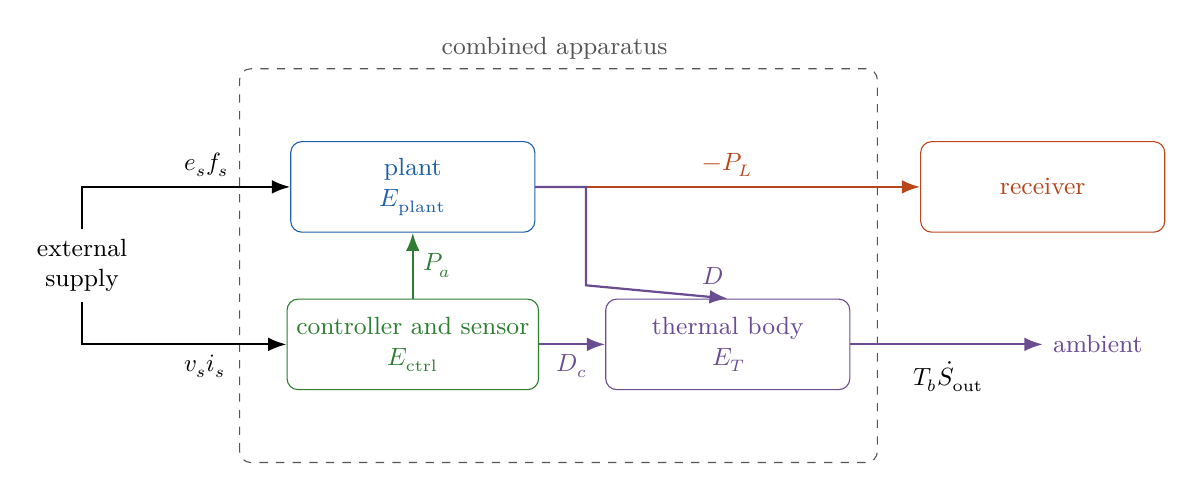
\begin{tikzpicture}[>=Latex,font=\small,
 box/.style={draw,rounded corners,minimum width=3.1cm,minimum height=1.15cm,align=center},
 arr/.style={->,thick}]
\draw[dashed,frameline,rounded corners] (-2.2,-2.5) rectangle (5.9,2.5);
\node[above,frameline] at (1.8,2.5) {combined apparatus};
\node[box,draw=elemA,text=elemA] (p) at (0,1) {plant\\$E_{\rm plant}$};
\node[box,draw=elemC,text=elemC] (c) at (0,-1) {controller and sensor\\$E_{\rm ctrl}$};
\node[box,draw=elemD,text=elemD] (h) at (4,-1) {thermal body\\$E_T$};
\node[box,draw=elemB,text=elemB] (r) at (8,1) {receiver};
\node[align=center] (s) at (-4.2,0) {external\\supply};
\draw[arr] (s) |- (p.west) node[pos=.8,above] {$e_sf_s$};
\draw[arr] (s) |- (c.west) node[pos=.8,below] {$v_si_s$};
\draw[arr,elemC] (c) -- (p) node[midway,right] {$P_a$};
\draw[arr,elemB] (p) -- (r) node[midway,above] {$-P_L$};
\draw[arr,elemD] (p.east) -- (2.2,1) -- (2.2,-.25) -- (h.north)
 node[pos=.75,above right] {$D$};
\draw[arr,elemD] (c) -- (h) node[midway,below] {$D_c$};
\draw[arr,elemD] (h.east) -- (8,-1) node[right] {ambient};
\node[below] at (6.8,-1.1) {$T_b\dot S_{\rm out}$};
\end{tikzpicture}
\end{document}
